%Made By Thomas Debelle
%Ajouté des Packages si nécessaires
\documentclass{report}
\usepackage[a4paper, total={6in, 9in}]{geometry}
\usepackage[utf8]{inputenc}
\usepackage[french]{babel}
\usepackage{graphicx}
\usepackage{graphics}
\usepackage[T1]{fontenc}
\usepackage{amsmath}
\usepackage{hyperref}
\usepackage{amssymb}
\usepackage{listings}
\usepackage{xcolor}
\usepackage{array}
\usepackage{float}
\usepackage{amsfonts}
\usepackage{fancyhdr}
\usepackage{titlesec}
\usepackage{xparse}
\usepackage{wrapfig}

\hypersetup{
    colorlinks=true,
    linkcolor=black,
    filecolor=magenta,
    urlcolor=cyan,
    pdftitle={Overleaf Example},
    pdfpagemode=FullScreen,
    }
\begin{document}

%Si la mention "Juin 2023" est sur une autre page, changé le dernier VSPACE
\begin{titlepage}
    \begin{figure}
        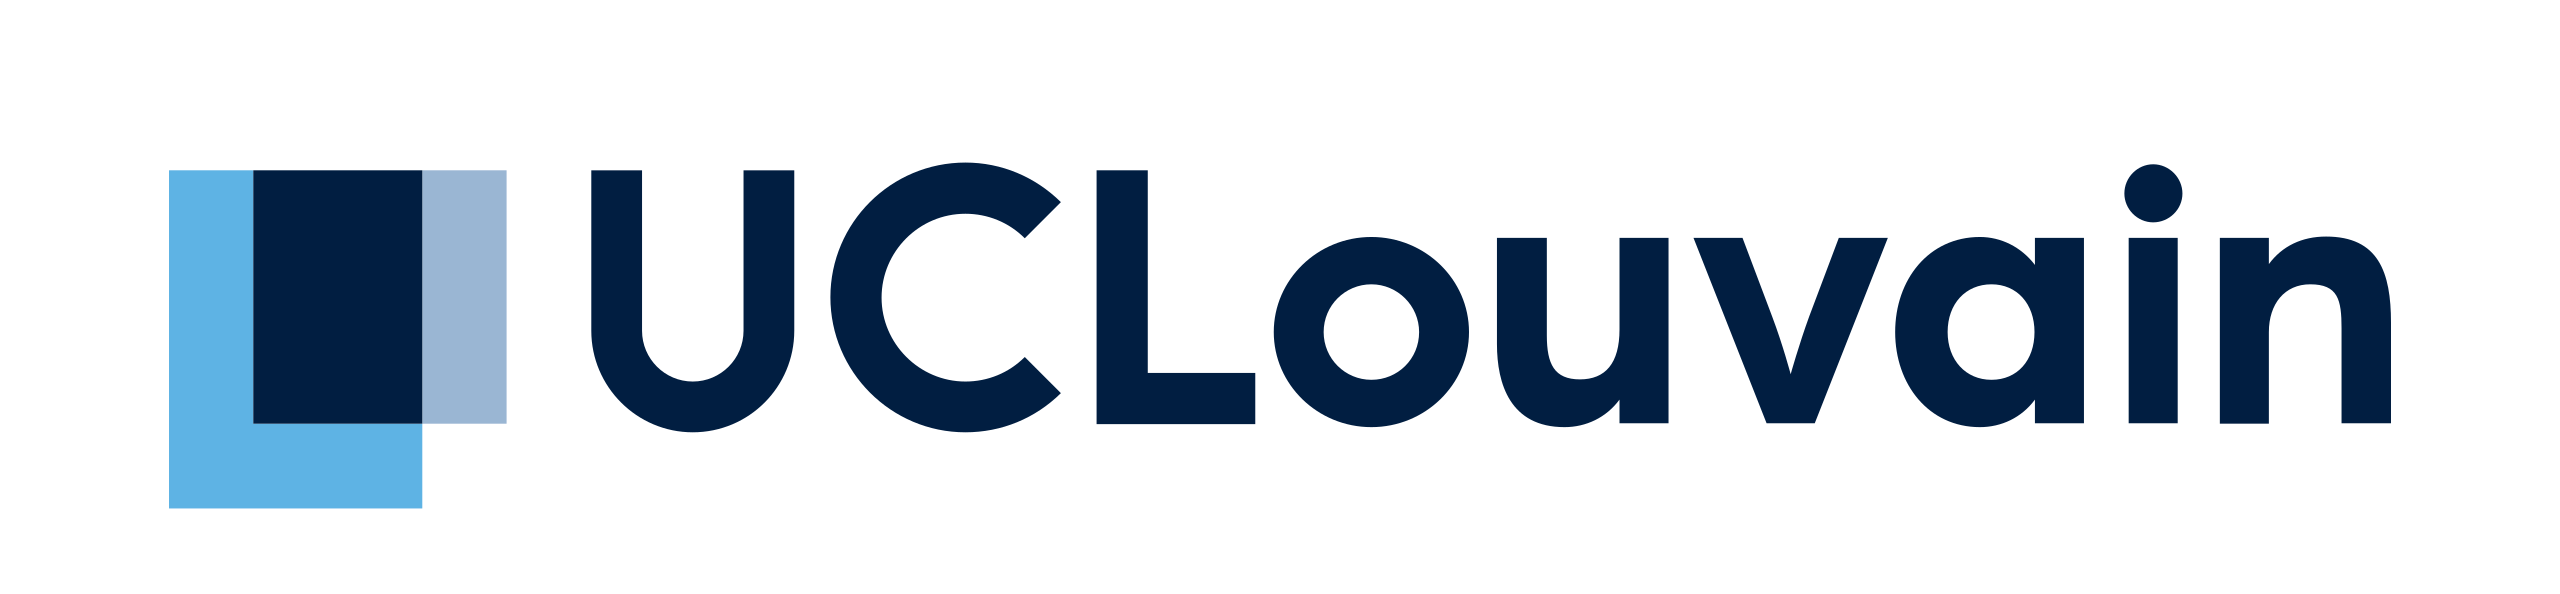
\includegraphics[height = 2cm]{UCL_Logo.png}
        \label{fig:my_label}
    \end{figure}

    \hspace*{100cm}
    \centering
    \vspace*{7cm}

    {\Huge \textbf{Résumé de LINFO1123}}\\
    \vspace*{0.25cm}
    compilation du \today\\
    \vspace*{0.25cm}
    \Large{Thomas Debelle}\\

    \vspace*{9.5cm} %Le dernier VSPACE
    {\Large Juin 2023}
\end{titlepage}

%_____NE PAS MODIFIER______
\setcounter{tocdepth}{1}
\tableofcontents
\newpage

\section*{Préface}

Bonjour à toi !\\

Cette synthèse recueille toutes les informations importantes données au cours, pendant les séances de tp et est amélioré grâce au note du Syllabus. Elle ne remplace pas le cours donc écoutez bien les conseils et potentielles astuces que les professeurs peuvent vous donner. Notre synthèse est plus une aide qui on l'espère vous sera à toutes et tous utiles.\\

Elle a été réalisée par toutes les personnes que tu vois mentionné. Si jamais cette synthèse a une faute, manque de précision, typo ou n'est pas à jour par rapport à la matière actuelle ou bien que tu veux simplement contribuer en y apportant ta connaissance ? Rien de plus simple ! Améliore la en te rendant \href{http://www.github.com/Tfloow/Q4_EPL}{ici} où tu trouveras toutes les infos pour mettre ce document à jour. (\textit{en plus tu auras ton nom en gros ici et sur la page du github})\\

Nous espérons que cette synthèse te sera utile d'une quelconque manière ! Bonne lecture et bonne étude.

%_______Vous pouvez modifier en-dessous_____
\chapter{Concepts}
Dans ce chapitre, on s'intéresse aux ensembles, cardinalité et équipotences de ces derniers
\section{Ensemble}
Un ensemble est un \textit{collection} d'objets, \textit{sans répétition}, ces derniers sont appelés \textit{éléments} de l'ensemble.
Donc un ensemble peut être des chiffres, des lettres, il peut être vide symbolisé par $void$ %à ajouter
On peut réaliser des opérations dessus, on peut déterminer des \textit{sous-ensembles d'ensemble} donc des ensembles issus d'ensemble.
On a également une notion s'appelant le \textit{complément} d'un ensemble dénoté $\tilde{A}$\\%trouver le bon charactère

\subsubsection{Langage}
Un \textit{langage} n'est autre qu'un mot ou bien un ensemble de caractères d'une taille fixée. Une chaine vide est écrite via le caractère "$\epsilon$".\\
On forme un langage via un \textit{alphabet} qui n'est autre qu'un ensemble de symboles, on le dénote "$\Sigma$". Tout langage est donc une suite de symbole issue de l'\textit{alphabet}.\\
$\Sigma^*$ correspond à l'ensemble des langages formés via l'alphabet.

\subsubsection{Relations}
Lorsque nous avons deux ensembles appelés \textit{A} et \textit{B}, on peut établir une relation appelé \textcolor{brown}{R} qui nous donne un sous-ensemble $AXB$ %trouver le symbole pour cross product
On peut représenter la relation par une table.

\subsubsection{Fonctions}
Lorsque nous avons deux ensembles appelés \textit{A} et \textit{B}, on peut avoir ce qu'on appelle une \textit{fonction} \textcolor{brown}{F}. C'est une relation tel que:
\begin{equation}
\exists a \in A : \exists b \in B :\quad <a,b> \quad \in f
\end{equation}
Il n'existe pas plus d'un b pour un a. Si pour un a il n'existe pas de b, on dit que $f(a)$ est indéfini et donc $f(a) = \perp$ ou \textit{bottom}.

\subsubsection{Propriétés des fonctions}
\begin{itemize}
\item un \textcolor{brown}{domaine de fonction} ou dom(f) $= {a \in A | f(a) \neq \perp}$
\item une \textcolor{brown}{image de fonciton} ou image(f) $= b \in B | \exists a \in A: b = f(a)$
\item f est dit \textcolor{brown}{fonction totale} si dom(f) $= A$
\item f est dit \textcolor{brown}{fonction partielle} si dom(f) $\in A$ % trouver le symbole pour include
\item f est \textcolor{brown}{surjectif} ssi image(f) = B autrement dit, tout élement est associé à minimum 1 élément dans B.
\item f est \textcolor{brown}{injectif} ssi $\forall a, a' \in A: a \neq a' \Rightarrow f(a)\neq f(a')$ autrement dit on ne fait correspondre qu'au plus un élément de A dans B.
\item f est \textcolor{brown}{bijectif} s'il combine \textit{surjectif} et \textit{injectif}
\end{itemize}

Intéressons nous aux \textcolor{red}{extensions} qui est le fait de rajouter une fonction qui ne définit un élément de B pas encore défini.
\begin{equation}
\forall x \in A : g(x) \neq \perp \Rightarrow f(x) = g(x)
\end{equation}	
f à la même valeur que g partout où g est défini.

\subsubsection{Définition d'une fonction}
Comme dit précédemment, une fonction est défini par sa table. On va souvent utiliser une description de la table qui permet que celle-ci soit clair et bien défini. De plus, on a pas besoin de savoir comment calculer ceci.\\
On peut également définir une table via une fonction ou un algorithme.

\section{Ensemble énumérable}
On dit que 2 ensembles ont le même cardinal (\textit{A} et \textit{B}) ssi il existe une bijection entre ces 2 ensembles. Donc chaque élément de \textit{A} correspond à un élément de \textit{B}.\\

On dit d'un ensemble qu'il est dénombrable ssi il est \textcolor{red}{fini} ou il existe une \textcolor{red}{bijection} entre l'ensemble $\mathbb{N}$ et cet ensemble.

\subsubsection{Exemples}
\begin{itemize}
\item L'ensemble $\mathbb{Z}$
\item L'ensemble des nombres pairs
\item Des paires d'entiers
\item L'ensemble des programmes Java
\end{itemize}

\subsubsection{Propriétés}
Tout sous-ensemble d'ensemble énumérable est \textit{énumérable}. L'union et l'intersection d'ensembles énumérables est \textit{énumérable}.\\

En s'intéressant à l'ensemble des programmes informatiques, on se rend compte que c'est une \textit{ensemble énumérable infini}. De plus, les programmes informatiques ne considèrent que des choses \textit{énumérables}.

\section{Cantor}
Le théorème de \textit{Cantor} nous dit que l'ensemble des nombres entre 0 et 1 compris est \textit{non énumérable}.
\begin{equation}
E = {x \in \mathbb{R} | 0 < x \le 1}
\end{equation}

\subsubsection{Preuve}
Pour prouver cela, on va réaliser une table et on va réaliser une \textit{diagonalisation de Cantor}.
\begin{center}
\begin{tabular}{|c||c|c|c|c|c|}
	\hline
	 & chiffre 1 & chiffre 2 & ... & chiffre $k+1$ & ...\\
	 \hline
	 $x_0$ & \textcolor{red}{$x_{00}$} & $x_{01}$ & ... & $x_{0k}$ & ...\\
	 \hline
	 $x_1$ & $x_{10}$ & \textcolor{red}{$x_{11}$} & ... & $x_{1k}$ & ...\\
	 \hline
	 ...& ... & ... & ... & ... & ...\\
	 \hline
	 $x_k$ & $x_{k0}$ & $x_{k1}$ & ... & \textcolor{red}{$x_{kk}$} & ...\\
	\hline
	 ...& ... & ... & ... & ... & ...\\
	\hline
\end{tabular}
\end{center}
Ensuite, on va définir notre nombre de la diagonale qui vaut $d = 0.x_{00}x_{11}...x_{kk}$. De cet valeur, on va créer une valeur $d'$ qui a comme propriété $x_{kk} \neq x'_{kk} \forall k$.\\
Mais, on doit stocker notre valeur $d'$ dans la table. On la stock à $p$ ce qui donne $d' = 0.x'_{p0}x'_{p1}... \textcolor{red}{x'_{pp}}$ mais à cause de la construction de $d = 0.x_{00}x_{11}...\textcolor{red}{x_{pp}}$. Par construction, $x'_{pp} \neq x_{pp}$ mais cela ne peut être respecté. Donc, \textbf{il n'y a pas} de \textit{bijection} des $\mathbb{N}$ vers cet ensemble. Donc cet ensemble est \textit{non énumérable}.

\subsubsection{Autre ensemble non énumérable}
\begin{itemize}
\item L'ensemble des $\mathbb{R}$.
\item L'ensemble des sous-ensemble de $\mathbb{N}$.
\item L'ensemble des chaines infinies de caractères d'un alphabet fini.
\item L'ensemble des \textit{fonctions} de $\mathbb{N}$ dans $\mathbb{N}$.
\end{itemize}
Chose intéressante à noter, comme on a une infinité non énumérable de fonctions $\mathbb{N}$ dans $\mathbb{N}$ et un nombre de programme informatique \textit{infini énumérable}. On ne peut résoudre tous les problèmes informatiques donc.

\chapter{Programmes calculables}
\section{Les algorithmes}
Un algorithme est un ensemble \textit{d'instructions} qui a pour but de produire un résultat. Donc un algorithme n'est \textcolor{red}{pas une fonction}. Il \textit{calcule} une fonction. Un algorithme n'est pas forcément un \textit{programme}, il peut être un \textit{organigramme}. C'est un \textit{ensemble fini d'instructions}. C'est une sorte de \textit{calculateur}. Ici, on va considérer nos algorithmes comme \textit{n'ayant pas de limite} de:
\begin{itemize}
\item Taille de données
\item Taille d'instructions
\item Taille de la mémoire, mais on a une utilisation finie.
\end{itemize}

\subsection{Calculabilité}
Avant de continuer, il faut définir la \textit{calculabilité} des algorithmes car sans \textit{formalisme}, les algorithmes sont non rigoureux, non exploitables.\\

Ici, on base cette notion sur celle des \textit{programmes informatiques}. (plus intuitif).
Ainsi, on possède \textbf{2 univers} celui des \textit{programmes informatiques} et celui des \textit{problèmes}. Pour être plus précis, on se base sur le \textcolor{brown}{langage Java} et on se limite au fonction $\mathbb{N} \rightarrow \mathbb{N}$. Ainsi pour les fonctions, on aura \textbf{1 entrée} et \textbf{1 sortie}. (on peut également généraliser ceci en disant que $\mathbb{N}^n \rightarrow \mathbb{N}$)

\section{Fonction calculable}
Une fonction est dite \textit{calculable} s'il existe un \textit{programme Java} recevant \textbf{1 donnée} étant un nombre $\in \mathbb{N}$ et la fonction va nous retourner la \textit{valeur} de $f(x)$ \textit{si} elle est défini.\\
Si le programme \textit{ne se termine pas} donc pas défini ou erreur d'exécution on dit que $f(x) = \perp$. On définit bien la notion de calculabilité sur \textit{l'existence d'un programme}. on a 2 types de fonctions
\begin{enumerate}
\item Fonction \textit{partielle} calculable: on a \textit{parfois} un résultat
\item Fonction \textit{totale} calculable: on peut \textit{toujours} calculé quelque chose.
\end{enumerate}

\subsection{Ensemble récursif}
Maintenant, on va essayer de déterminer la calculabilité sur \textit{un ensemble de fonctions}.
Le principe de décision de \textit{calculabilité} est le principe dit \textit{récursif}.\\
\textbf{A} est \textcolor{red}{récursif} si il existe un programme \textit{Java} qui recevant n'importe quelle donnée sous forme d'un $\mathbb{N}$ fourni comme résultat:
\begin{itemize}
\item 1 si $x \in A$
\item 0 si $x \notin A$
\end{itemize}
Donc on est face à un \textit{algorithme} qui calcule si $x$ est dans A ou non. C'est un algorithme complet et se termine toujours. (attention de ne pas confondre \textit{récursif} et \textit{récursivité})\\

On dit qu'un ensemble d'algorithme est \textcolor{red}{récursivement énumérable} s'il est \textit{récursif} sauf qu'il retourne $\neq 1 \quad x \notin A$ ou ne se termine pas et qu'on puisse énuméré cet ensemble.

\subsubsection{Fonctions caractéristiques} \label{caract}
Une fonction caractéristique de $A \subseteq N$ et:
\begin{align}
X_A : N \rightarrow N : X_A(x) &= 1 \text{ si } x \in A\\
&= 0 \text{ si } x \in A
\end{align} 
C'est une autre manière de déterminer si un ensemble est récursift si $X_A$ est une fonction \textit{calculable}.\\
On dit qu'une fonction est récursivement énumérable ssi il existe une fonction f calculable ayant pour domaine A. Ou bien, on dit que A est vide \textit{ou} l'image de f est A ayant une fonction f \textit{totale} calculable.\\
Un \textcolor{red}{ensemble récursivement \textit{énumérable}} est un ensemble dont la bijection des $\mathbb{N}$ est énumérable et calculable.

Propriétés:
\begin{itemize}
\item A récursif $\Rightarrow$ A récursivement énumérable 
\item A récursif $\Rightarrow$ (N \ A) récursivement énumérable 
\item A récursif $\Rightarrow$ (N \ A) récursif 
\item A récursivement énumérable et (N \ A) récursivement énumérable $\Rightarrow$ A récursif 
\item A fini $\Rightarrow$ A récursif
\item (N \ A) fini $\Rightarrow$ A récursif
\item A récursif $\Rightarrow$ $\bar{A}$ récursif
\end{itemize}

\section{Thèse de Church-Turing}
Comment démontrer qu'une fonction \textbf{n'est pas} calculable.\\
Les 4 grands points de la thèse:
\begin{enumerate}
\item Aucun modèle de la notion de fonction calculable n’est plus puissant que les Machines de Turing (ici Java)
\item Toute fonction calculable (au sens intuitif) est calculable par une machine de Turing (ici Java)
\item Toutes les définitions formelles de la calculabilité connues à ce jour sont équivalentes (Théorème)
\item Toutes les formalisations de la calculabilité établies par la suite seront
équivalentes aux définitions connues
\end{enumerate}
On établit que Java à accès à une infinité de mémoire (donc physiquement possible). Ainsi, on a $P$ qui est l'ensemble des programmes Java syntaxiquement corrects, qui reçoivent 1 données \textit{entières} et qui retournent un résultat \textit{entier}.
\begin{itemize}
\item P est un ensemble récursif (infini dénombrable)
\item $P = P_0, P_1, ..., P_k, ...$ sans répétition donc chaque programme est unique.
\item Pour simplifier, $f(k) = P_k$
\item f est calculable.
\item k et $P_k$ représente le même objet
\end{itemize}

donc on dit que $P_k$ donne le programme $k$ dans l'ensemble $P$. on dit que $\varphi_k$ est la fonction mathématique calculé par $P_k$. Donc on peut avoir $\varphi_m == \varphi_n$ car réalise le même travail mais sont issues de programmes \textit{différents}. $\varphi_k: N \rightarrow N$. 

\section{Non calculabilité}
Pour rappel:
\begin{itemize}
\item Nombre de fonctions de $\mathbb{N} \rightarrow \mathbb{N}$ est \textbf{non} dénombrable.
\item Nombre de programmes Java est dénombrable.
\end{itemize}
En programmation, on s'intéresse aux fonctions définies de manière finie, donc on a une \textcolor{red}{infinité dénombrable}. Mais si une fonction est définie de manière finie, peut-elle être calculable ?

\subsection{Problème de l'arrêt}
Une fonction prends 2 paramètres: halt: P x N. P est le numéro du programme et N est son entrée.\\
\begin{align}
\text{halt}(n,x) &= 1 \text{ si } \varphi_n(x) \neq \perp\\
&= 0 \text{ sinon}\\
\text{halt}(n,x) &= 1 \text{ si l'exécution du } P_n \text{ se termine}\\
&= 0 \text{ sinon}
\end{align}
On a donc une table finie, mais décrite de manière finie donc bien définie. Peut-on la calculer ?

\subsubsection{Preuve par l'absurde} 

\begin{center}
\begin{tabular}{|c|c|c|c|c|c|}
\hline
& $0$ & $1$ & ... & $k$& ...\\
\hline
$P_0$ & \textcolor{red}{halt(0,0)} & halt(0,1) & ... & halt(0,k) & ...\\
\hline
$P_1$ & halt(1,0) & \textcolor{red}{halt(1,1)} & ... & halt(1,k) & ...\\
\hline
... & ... & ... & ... & ... & ... \\
\hline
$P_k$ & halt(k,0) & halt(k,1) & ... & \textcolor{red}{halt(k,k)} & ...\\
\hline
... & ... & ... & ... & ... & ... \\
\hline
\end{tabular}
\end{center}

On va sélectionner les valeurs sur la diagonale et stocker cela comme une variable s'appelant "\textit{diag}". On va donc modifié cette valeur et est représenté par "\textit{$diag_{mod}$}" qui inverse chaque nombre. (donc $0 \rightarrow 1$ et $1 \rightarrow 0$) Donc \textit{$diag_{mod}$} est calculable sous l'hypothèse que la fonction "halt" l'est.\\

Donc, il existe un programme Java qui calcule cette "$diag_{mod}$" qu'on trouvera en ligne $d$. Mais à cause de cela, $diag_{mod}(d) \neq diag(d)$ donc ne peut exister par \textit{définition}.\\

En conclusion, la fonction "halt" \textbf{n'est pas} calculable.

\subsubsection{Conclusion}
\begin{itemize}
\item  Aucun algorithme ne permet de déterminer pour tout programme Pn et donnée x si Pn(x) se termine ou non
\item Seule possibilité serait d’avoir un langage de programmation dans lequel tous les programmes se terminent. La fonction halt est alors calculable pour les programmes de ce formalisme
\item halt non calculable ne signifie pas que pour un programme k donné, halt(k,x) est
non calculable
\end{itemize}
Pour le premier point, on ne peut séparer le soucis en 2 algorithmes car on ne peut changer de programmes selon l'input. Un algorithme donne le \textbf{bon résultat} en fonction du résultat.\\

On dit que halt n'est pas calulable dans le sens où il n'existe pas d'algorithmes \textbf{généraux}.

\subsubsection{Exemple non-récursif}

\begin{align}
Halt &= \{(n,x) | \text{ halt}(n,x) = 1\}\\
&= \{(n,x) | P_n (x) \text{ se termine}\}\\
K &= \{n | (n,n) \in \text{HALT}\}\\
&= \{n | halt(n,n) = 1\}\\
&= \{n | diag(n) = 1\}\\
&= \{n | P_n(n) \text{ se termine}\}\\
\end{align}
Donc K et HALT \textbf{ne sont pas} récursifs mais sont récursivement énumérable car si un élément n'appartient pas à K ou HALT, il va boucler mais fournir la bonne solution s'il appartient à ces ensembles.\\
De plus K est la diagonale de \textit{HALT}.

$\overline{HALT}$ n'est pas récursivement énumérable car on a pas de moyen de prouver qu'un probable n'appartient pas à cet ensemble. pareil pour $\overline{K}$

\begin{figure}[H]
\centering
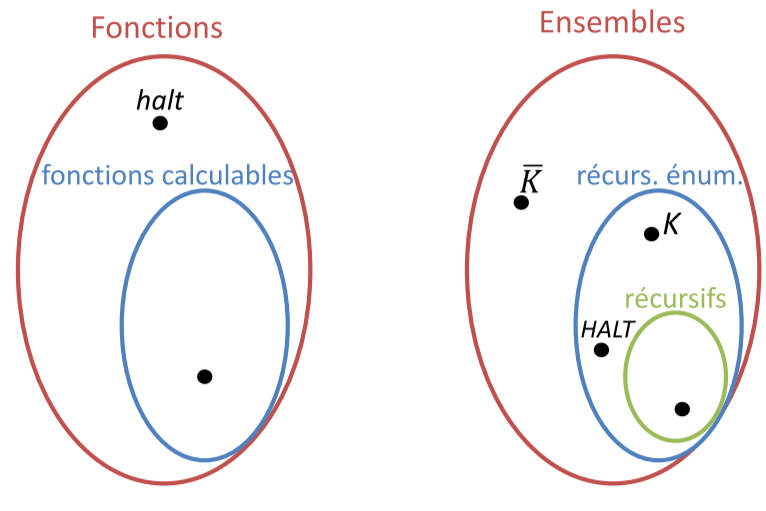
\includegraphics[width=5cm]{img/ensembleFonction.png}
\caption{Schématisation des fonctions et ensembles de fonctions}
\end{figure}

Le fait de ne pas pouvoir calculer "halt" nous pose soucis et va ouvrir tout un pan de soucis et limitations.\\

De plus, on peut faire face à des ensembles \textbf{co-récursivement} énumérable. En effet, il existe des ensembles co-récursivement énumérable tel que: $\overline{\textbf{K}}$ et tous les ensembles \textit{récursifs}. \label{coreq}

\section{Insuffisance des fonctions totales}
Pourquoi est-ce utile d'avoir un programme qui tourne en \textit{boucle}? N'avons-nous pas besoin de fonctions qui donnent un résultat précis tout le temps donc \textit{totale}?

Imaginons que nous créons un \textit{langage de programmation} qui a que des fonctions totales.
Donc, \textbf{Halt} est calculable et on a une réponse pour toutes fonctions. Halt serait la fonction constante 1.

Notre langage \textit{Q} est calculable donc ayant un interpréteur calculable.

\subsection{Théorème de Hoare-Allison} \label{HA}
Donc en résumé de notre langage \textit{Q}:
\begin{itemize}
\item L'interpréteur de ce programme est calculable
\item La fonction \textit{halt} est totale et correspond à la fonction constante de 1.
\item Mais l'interpréteur \textcolor{red}{n'est pas} calculable \textit{dans Q}.
\end{itemize}

\begin{center}
\begin{tabular}{|c|c|c|c|c|c|}
\hline
& $0$ & $1$ & ... & $k$& ...\\
\hline
$Q_0$ & \textcolor{red}{interpret(0,0)} & interpret(0,1) & ... & interpret(0,k) & ...\\
\hline
$Q_1$ & interpret(1,0) & \textcolor{red}{interpret(1,1)} & ... & interpret(1,k) & ...\\
\hline
... & ... & ... & ... & ... & ... \\
\hline
$Q_k$ & interpret(k,0) & interpret(k,1) & ... & \textcolor{red}{interpret(k,k)} & ...\\
\hline
... & ... & ... & ... & ... & ... \\
\hline
\end{tabular}
\end{center}
La colonne \textit{Q} correspond à l'ensemble des programmes et la ligne de nombre correspond aux entrées de chaque programme.

Tous les programmes se terminent donc \textit{jamais} $\perp$. On sélectionne la diagonale:
\begin{align}
diag(n) &= interpret(n,n)\\
diag_{mod}(n) &= interpret(n,n) + 1\\
Q_l &= diag_{mod}
\end{align}
Et donc, on voit facilement que à la ligne $l$ il y aura un souci avec $diag$ et notre entrée à $Q_l$ qui n'est autre que $diag_{mod}$. en effet $diag_{mod}(l) \neq diag(l)$. Donc la fonction \textit{interpret} n'est \textbf{pas} calculable en \textit{Q}.\\

Le \textit{théorème} nous dit donc que: Si un langage de programmation (non trivial) ne permet que le calcul de fonctions totales, alors: 
\begin{itemize}
\item l’interpréteur de ce langage n’est pas programmable dans ce langage 
\item il existe des fonctions totales non programmables dans ce langage
\item ce langage est \textcolor{red}{restrictif}
\end{itemize}

Donc si on peut faire un interpréteur d'un langage dans son langage, la fonction \textit{halt} n'est pas totale. Donc c'est soit programmable par lui-même soit fonction totale de halt.\\

Si on veut qu’un langage de programmation permette la programmation de toutes les fonctions totales calculables, alors ce langage doit également permettre
la programmation de fonctions non totales.\\

De plus, si on avait une fonction qui regarde si des fonctions sont totales, cela pose problème. Cela est impossible et donc cette fonction $tot(n)$ n'est pas récursif.

\subsection{Interpréteur}
Pour qu'un formalisme soit assez puissant, il faut que ce dernier arrive à programmer son propre interpréteur.

\begin{equation}
\exists z \forall n,x : \varphi_z(n,x) = \varphi_n(x)
\end{equation}
Avec $\varphi_z$ qu'on appelle la fonction universelle. et $P_z$ est le programme universel. Par convention, on appelle $\theta(n,x)$ la \textcolor{red}{fonction universelle}.

\section{Extension des fonctions partielles}
Pour l'instant, nous n'avons vu que des fonctions qui soit donnent le bon résultat soit donne $\perp$ et donc boucle. On va réaliser des \textit{extensions}, c'est-à-dire que nous allons retourner la valeur correcte dans les cas possible et un message ou autre chose pour le reste des entrées.\\

Un \textit{théorème} nous dit que, \textit{Il existe une fonction partielle calculable g telle qu’aucune fonction totale calculable n’est une extension de g}.\\
Pour prouver cela, on utilise la fonction \textit{nbstep(n,x)} qui correspond au nombre d'instruction avec l'arrêt de $P_n(x)$. ($P_n(x) = \perp$)La preuve se fait pas diagonalisation comme avant (\href{http://ezcast.uclouvain.be/ezplayer/index.php?action=view_asset_bookmark&album=LINFO1123-pub&asset=2021_02_17_21h51_34s&t=224&type=cam&token=EVKUMNQV}{vidéo}).\\

\section{Théorème de Rice}
\subsection{Réduction à Halt}
Pour montrer que f(x) est non calculable on suppose que:
\begin{itemize}
\item f(x) est calculable.
\item Sous cette hypothèse la fonction halt(n,x) est alors calculable.
\item Comme halt(n,x) est enfaite non-calculable, f(x) est également non-calculable.
\end{itemize}

\subsubsection{Raisonnement}
Définissons une fonction qui dit que:
\begin{align*}
f(n) &= 1 \quad \text{ si } \varphi_n(x) = \perp\\
&= 0 \quad \text{ sinon}
\end{align*}
On suppose que $f(n)$ est calculable et on veut montrer que halt est calculable. Pour se faire:
\begin{enumerate}
\item On \textcolor{red}{construit} (pas exécute) un programme qui dit: $P(z) \equiv P_n(x); print(1)$
\item On obtient le numéro de programme: $d = \text{ numéro de programme } P(z)$
\item On regarde si le résultat de cette fonction calculable pour créer halt:
\begin{lstlisting}[escapechar=\%]
if F(d) = 1 then
	print(0) %//\textit{car on est bottom et cela boucle}%
else
	print(1) %//\textit{car le programme se termine}%
\end{lstlisting}
\item Donc on en conclue que cette fonction halt est non-calculable
\end{enumerate}
On utilise ce type de démarche pour tout autre fonction du même genre. (on doit impérativement définir le comportement de la fonction)

\subsection{Théorème}
On s'intéresse à comparer des programmes entre eux, savoir si un programme est correct.
\subsubsection{Idée de base}
Dans l'ensemble des programmes, on va séparer cet ensemble en 2 \textit{sous-ensembles}.
\begin{figure}[H]
\centering
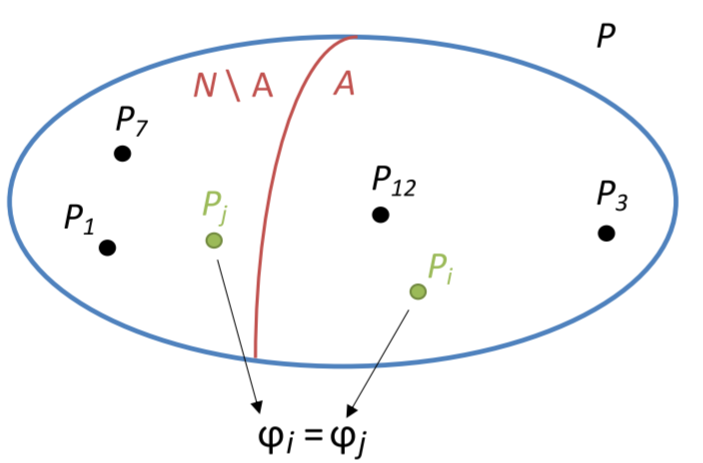
\includegraphics[width=6cm]{img/rice.png}
\end{figure}
On a que:
\begin{align*}
\text{Soit } A &\subseteq \mathbb{N}\\
\text{Si } A \text{ récursif et } A \neq \varnothing &\text{ et } A \neq \mathbb{N}\\
\text{Alors } \exists i \in A &\text{ et } j \in \mathbb{N} \setminus A : \varphi_i = \varphi_j 
\end{align*}
Ce qui revient à dire que:
\begin{align*}
\text{Si } \forall i \in A &\text{ et } \forall j \in \mathbb{N} \setminus A: \varphi_i \neq \varphi_j\\
\text{Alors } A \text{ non récursif \textit{ou} } &A = \varnothing \text{ ou } A = \mathbb{N}
\end{align*}
De plus, si un programme est récursif, on peut savoir de quel ensemble il est.

\subsubsection{Compréhension}
\begin{enumerate}
\item \textcolor{red}{Si} une propriété de programmes, vérifiée par certains programmes mais pas tous, est décidable, \\
\textcolor{red}{alors} il existe deux programmes équivalents (calculant la même fonction) dont un vérifie la propriété et l’autre pas
\item \textcolor{red}{Si} une propriétéde la fonctioncalculée par un programme est vérifiée par certains programmes, mais pas par tous, \\
\textcolor{red}{alors} cette propriété ne peut être décidée par un algorithme
\item \textcolor{red}{S'il} existe un algorithme permettant de déterminer si un programme quelconque calcule une fonction ayant cette propriété, \\
\textcolor{red}{alors} toutes les fonctions calculables ont cette propriété ou aucune fonction
calculable n’a cette propriété
\end{enumerate}
Voyons plus en détail ce que chacun veule dire:
\begin{enumerate}
\item C'est une simple traduction du théorème en français.
\item Cela signifie qu'on ne peut pas vérifier si 2 programmes sont équivalents !
\item Autre façon d'énoncer le théorème de \textit{Rice}.
\end{enumerate}

\subsection{Exmple}
Commençons avec: $ A_1 = \{i | \varphi_i \text{ est totale}\}$ ($P_i$ s'arrête toujours)\\
Donc on sait que $A_1 \neq \varnothing$ car on a une fonction $P_k(x) \equiv print(1)$ et on sait ainsi que $k \in A_1$. Ce n'est pas $A_1 \neq \mathbb{N}$ car $P_l(x) \equiv while true$ n'est pas total ! De plus, notre ensemble $A$ a des fonctions totales et l'ensemble $\overline{A}$ des fonctions non-totales, par construction: $\forall i \in A \text{ et } \forall j \in \mathbb{N}: \varphi_i \neq \varphi_j$\\

Via le théorème de \textit{Rice}, $A_1$ est un ensemble non-vide et non égale à $\mathbb{N}$. On a également prouvé que les fonctions ne sont pas égales entre les 2 \textit{ensembles}. On en \textit{conclut} que l'enseble \textbf{n'est pas récursif}.

\subsection{Analyse du théorème}
Bonne nouvelle, on est pas remplaçable (ou presque).
\begin{enumerate}
\item Aucune question relative aux programmes, vus sous l’angle de la \textbf{fonction} qu’ils calculent, ne peut être décidée par l’application d’un algorithme
\item Les propriétés intéressantes d’un programme concernent la fonctionqu’il calcule, nonpas la forme (syntaxe) du programme
\item La plupart des problèmes intéressants au sujet des programmes sont non
calculables
\end{enumerate}
Mauvaise, on ne peut pas automatiser qu'un programme est correct.

\subsection{Démonstration}
Supposons que $A \neq \varnothing$ et $A \neq \mathbb{N}$. Et on suppose que $\forall i \in A, \forall j \in \overline{A}: \varphi_i \neq \varphi_j$ Donc $A$ ne peut être récursif. On va \textbf{démontrer} cela.\\

Pour prouver cela on va utiliser une réduction à \textit{halt}. On fait les choses suivantes:
\begin{enumerate}
\item On suppose que $A$ est récursif.
\item Donc halt est calculable mais ce n'est pas le cas.
\item Donc est n'est pas récursif.
\end{enumerate}
On va donc séparer notre ensemble des Programmes et on effectue ces manipulations:
\begin{enumerate}
\item $\mathbb{N}$ en $A$ et $\overline{A}$. On dit que $P_k(x) \equiv while true$ et que $k \in \overline{A}$
\item On sait que $A \neq \varnothing, \exists m \in A$ (on sait que c'est différent du vide donc il existe au moins 1 programme quelconque)
\item On peut affirmer que (par hypothèse de récursif) $\varphi_k \neq \varphi_m$
\item On crée un programme pour \textit{halt}:
	\begin{itemize}
	\item On construit: $P(z) \equiv P_n(x); P_m(z)$
	\item On assigne un numéro de programme qu'on a construit: $d = \#P(z)$. Cela dépend de ma donnée $n$ et $x$.
	\item on exécute un programme qui regarde si $d \in A$ il print $1$ qu'il appartient sinon il imprime $0$.
	\end{itemize}
\item On exécute le programme: si $P_n(x)$ se \textbf{termine} alors $\varphi_d = \varphi_m$. \textbf{Sinon} il boucle et est $\varphi_d = \varphi_k = \perp$
\item Donc aucun programme dans $A$ et $overline{A}$ n'est équivalent. Donc tester que $\varphi_d = \varphi_m$ est la même chose que tester que $d \in A$ et inversement.
\item Donc, \textcolor{red}{Halt est non calculable} car il boucle, donc A est bien \textbf{non récursif}.
\end{enumerate} 


\section{Théorème de la paramétrisation}
De manière générale, une fonction peut être vu comme $f: N \rightarrow N$ mais \textit{également} comme $f: P \rightarrow P$. Donc $f(a) = b$ et en combinant $P_a = P_B$ notre $f$ devient un \textbf{transformateur de programmes}. Pour être plus précis c'est le $P_k$ qui calcule $f$ qui est le \textit{transformateur de programmes}.

\subsection{Théorème S-m-n via S-1-1}
On dit qu'il existe une fonction calculable qui prend 2 arguments tel que:
\begin{align*}
S_1^1 : N^2 &\rightarrow N \text{ et } \forall k\\
\varphi_k^{(2)} (x_1, x_2) &= \varphi_{S_1^1 (k,x_2)} (x_1)
\end{align*}
\subsubsection{Compréhension}
On dit qu'il existe un \textit{transformateur} ($S_1^1$) qui prend en arguments: - Un programme à 2 arguments et 1 valeur $v_2$\\
Cela donne comme résultat un programme $P(x_1)$ qui calcule la même chose que $P_k(x_1,v_2)$.

\subsection{Via S-m-n}
On dit que:
\begin{align*}
\forall m, n \geq 0 &, \exists S_n^m : N^{m+1} \rightarrow N : \forall k\\
\varphi_k^{n+m} (x_1, ..., x_n, x_{n+1}, ..., x_{n+m}) &= \varphi_{S_n^m (k, x_{n+1}, ..., x_{n+m})}^{(n)} (x_1, ..., x_n)
\end{align*}
\subsubsection{Compréhension}
Comme nous avons $m,n \geq 0$, il existe un transformateur de programmes appelés $S_n^m$ qui reçoit: - $P_k$ avec $m+n$ arguments, $m$ valeurs $v_1, ..., v_m$\\
Cela renvoi comme résultat un programme P à $n$ arguments. Donc $P(x_1, ..., x_n)$ calcule la \textit{même} fonction que $P_k(x1, ..., x_n, x_{n+1}, ..., x_{n+m})$



\textcolor{red}{TODO section 10 et 11}

\section{Autre problèmes non calculables}
\subsubsection{Liste équivalente de mot}
Si on a 2 listes comme ci-dessous, il n'existe \textbf{aucun} algorithme qui nous permettent de trouver une suite d'indice qui produit 2 mots équivalents depuis deux listes. C'est donc un problème \textbf{non calculable}.
\begin{lstlisting}[escapechar=\%]
%$\Sigma$% = {a,b} 
U = {u1=b, u2=babbb, u3=ba}
V = { v1=bbb, v2=ba, v3=a}
Res = {2 1 1 3} //%car U: babb, b, b, ba et V: ba, bbb,bbb, a%
\end{lstlisting}

\subsubsection{Équations diophantiennes}
C'est une équation de la forme: $D(x_1, ..., x_n) = 0$. L'équation ne possède que des \textit{coefficients entiers} et on cherche des solutions \textit{entières}.\\
C'est bel et bien un problème \textbf{non calculable}.
\begin{align*}
P(a) \leftrightarrow \exists x_1, ..., x_n [D(a,x_1, ..., x_n) = 0]
\end{align*}
Ci-dessus, c'est la condition pour être diophantien pour une fonction.

\section{Codage et représentation}
Jusqu'ici, on avait des fonctions $N^n \rightarrow N$ et on avait des représentations décimales des nombres. Mais on ne prend pas en compte les autres types de donnés, ... Donc on va créer des fonctions de codage et représentation.

\subsubsection{Codage}
On va définir une bijection entre notre nouveau type et les entiers. On peut identifier chaque objet par un entier \textit{distinct}. Ce qui nous amène à une propriété très utile:
\begin{enumerate}
\item la fonction de codage est bijective
\item la fonction de codage est calculable
\item la fonction de codage inverse est calculable
\end{enumerate}

\subsection{Les nombres calculables}
On sait que tout nombre réel est fini tout comme la limite d'une suite \textit{convergente} vers un rationnel $\mathbb{Q}$ Donc:
\begin{align*}
\forall x \in \mathbb{R}, \exists s &: N \rightarrow Q : \text{ (s est total)}\\
lim_{n\rightarrow \infty} &| x - s(n)| = 0
\end{align*}

\subsubsection{Définition}
On dit qu'un réel $x$ est \textbf{calculable} si il existe une \textcolor{red}{fonction totale calculable}:
\begin{align*}
s: N \rightarrow Q\\
\forall n: |x-s(n)| \leq 2^{-n}
\end{align*}
Donc notre fonction ne fait que s'approcher autant qu'on veut de notre réel.

\subsubsection{Propriétés}
Donc un $\mathbb{R}$ est calculable s'il existe un programme qui le calcule. Ce qui par induction rend l'ensemble des nombres calculables énumérables.\\
Il existe des réels donc non-calculables mais qui peuvent être définie de manière finie comme:
\begin{align*}
x = \sum_{0 \geq n \geq \infty} \chi_K (n) 3^{-n}
\end{align*}


\chapter{Modèles de calculabilité}

\section{Familles de modèles}
\noindent 
Il existe \textcolor{red}{2} familles de modèles:
\begin{enumerate}
\item Basé sur le \textcolor{red}{calcul}
\item Basé sur le \textcolor{red}{langage} (chaine de caractère)
\end{enumerate}

\subsection{Basé sur le calcul}
Leur objectif est de modéliser le concept de fonctions calculables, processus de calcul, algorithme effectif, ... Ex
\begin{itemize}
\item Automate fini
\item Machine de Turing
\item Langages de programmation
\end{itemize}
Il existe 2 sous-catégories:
\begin{enumerate}
\item Modèles \textcolor{blue}{déterministes}: il n'y a qu'un seule exécution possible d'un programme pour un input donné.
\item Modèles \textcolor{blue}{non déterministes}: il existe plusieurs exécutions possibles pour un input donné.
\end{enumerate}

\subsection{Langes de programmation}
C'est le modèle basé sur le \textcolor{red}{calcul} qui est un exemple de la \textbf{calculabilité} qui est le plus \textit{courant}. (on l'a utilisé pour démontrer toutes les théories fondamentales de la \textit{calculabilité})

\subsubsection{Définir un langage}
\noindent
On doit définir la:
\begin{enumerate}
\item Syntaxe du langage
\item Sémantique du langage
\item Convention de représentation d'une fonction par un programme
\end{enumerate}

\subsubsection{Équivalence des programmes}
On sait que les langages de programmation sont \textcolor{blue}{équivalents} entre eux. Tous sont équivalents. Une fonction est calculable en \textit{Rust} alors il sera calculable en \textit{C}. On dit que les langages sont \textcolor{red}{Complets}.\\
Bien évidemment, certains problèmes sont plus simples et/ou plus efficace dans un langage de programmation.\\

\subsubsection{BLOOP}
BLOOP ou \textit{Bounded loop} qui est Java sans les boucles while, on ne modifie pas la variable de \textit{compteur} dans le corps d'un \textit{for}. Pas de méthodes récursives ni mutuellement récursibles.\\
Donc \textcolor{blue}{BLOOP} se termine toujours et ne calcule que des fonctions \textit{totales}. Cependant, il ne calcule pas \textcolor{red}{toutes les fonctions totales} (voir \ref{HA}). En effet, l'interpreteur n'est pas programmable en BLOOP. Donc ce \textbf{n'est pas} un modèle complet de la calculabilité.

\subsection{Non-déterministe}
On va créer \textcolor{blue}{ND-Java} qui est une version \textit{non-déterministe} de Java. On lui ajoute la fonction \textbf{choose(n)} qui renvoie un entier entre \textbf{0 et n} et est donc non déterministe.\\
On doit considérer n+1 exécution possible à chaque lancement de la fonction. \\
Donc pour le problème du voyageur de commerce, on va énumérer tous les chemins possibles en swapant un à un les villes. Donc on aura un arbre de décision. Ainsi, on peut regarder la profondeur du chemin pour savoir si le nombre de possibilité est borné.\\
Il y aura des chemins où ce sera borné et des chemins où ça ne l'est pas.\\
On dit qu'un programme nous produit une \textcolor{blue}{relation} plutôt qu'une fonction.

\subsubsection{Récursif ND}
On dit qu'un ensemble A ($A \in \mathbb{N}$) est \textcolor{red}{ND-récursif} si il existe un programme \textbf{ND-Java} tel que lorsqu'il reçoit comme donnée n'importe quel nombre nature $x$.
\begin{itemize}
\item si $x \in A$, alors il existe un \textcolor{blue}{exécution} fournissant comme résultat 1 (peu importe le temps)
\item si $x \notin A$ alors \textbf{toutes} les \textcolor{blue}{exécutions} possibles fournissent comme résultat 0.
\end{itemize}

\subsubsection{ND Récursivement énumérable}
On dit que A est \textcolor{red}{ND-récursivement énumérable} si il existe un programme ND-Java tel que lorsqu'il reçoit comme donnée n'importe quel nombre naturel x, il existe une \textcolor{blue}{exécution} fournissant comme résultat 1 \textbf{ssi $x \in A$}. (Si $x \notin A$ alors la fonction retourne autre chose que $1$ ou est $\perp$)

\subsubsection{Propriétés}
Un ensemble est \textbf{ND-récursif} ssi il est \textbf{récursif}. Si nous avons un arbre d'exécutions possibles, il est toujours possible de parcourir tous les \textbf{étages} de notre arbre et donc parcourir toutes les exécutions \textcolor{blue}{possibles}.\\
Si la profondeur d'une branche est de taille $n$, alors mon parcours a une complexité exponentielle tel que $b^n$.

\subsection{Basé sur le langage}

Se base sur un ensemble de mot et possède une \textcolor{blue}{grammaire formelle}. On essaye de modéliser une classe de langages. Le langage est donc un ensemble \textit{récursif} ou \textit{récursivement énumérable}. Pas vu dans ce cours

\section{Automates finis}
\noindent
C'est une modélisation assez simple du concept de \textit{calcul}, il y a:
\begin{itemize}
\item Un nombre \textit{fini d'états}
\item Une lecture d'une donnée: un mot
\item Chaque symbole de la donnée est lu \textit{une et une seule} fois
\item On transitionne d'état en étant en fonction du \textit{symbole lu}.
\item L'état final est l'état après avoir \textit{lu tous les symboles} de la donnée
\item On \textbf{ne peut pas} mémoriser quelque chose. 
\end{itemize}
Donc l'objectif d'un \textcolor{blue}{automate fini} est de \textbf{décider} si un mot appartient à un langage. Réponse binaire: Oui ou Non. Pas de boucle.
\subsubsection{Modèle}
\noindent
On a un:
\begin{itemize}
\item $\sum$ qui est l'ensemble (\textit{fini}) de symboles
\item $S$ qui est l'ensemble (\textit{fini}) d'états
\item $s_0 \in S$ qui est l'état initial
\item $A \subseteq S$ qui est un ensemble d'état acceptant
\item $ \delta  S  \Sigma \rightarrow S $ qui est une fonction de \textit{transition}. (C'est une sorte de tableau)
\end{itemize}
C'est donc un modèle de calcul. On parcourt le mot symbole par symbole et on termine notre exécution à la fin de la lecture de symbole. Pour simplifier tout cela, on va rajouter un état \textit{fail} si on n'a pas tout déterminé pour les multiples possibilités.\\

Un état acceptant est représenté par un \textbf{double cercle} et un état non-acceptant est représenté par un \textbf{simple cercle}. Les flèches ou les \textit{arcs} sont les \textcolor{blue}{fonction de transition}.\\

Un mot est accepté si l'état finale de ce mot est dans l'état \textit{acceptant}. (et vice-versa)\\
Dans un automate fini, son exécution se finit \textbf{toujours}! Donc cela ne détermine que des ensembles \textcolor{blue}{récursifs} (mais pas tous les ensembles récursifs (\ref{HA}))

\subsection{Extension}
On peut étendre les automates aux \textcolor{blue}{automates finis non déterministes}. On a donc plusieurs transitions possibles pour une paire. Plusieurs exécutions pour une même donnée.\\
Un mot m est accepté par \textit{NFDA} si il existe \textbf{une} exécution de NFDA, on finit dans un état acceptant.\\
Pour toute exécution de NFDA, un mot \textbf{n'est pas accepté} s'il ne tombe jamais sur un état acceptant.\\

On peut voir comme si on rassemblait des exécutions ensemble et des ensemble d'états. \\

\subsubsection{Avec transitions vides}
On peut faire des transitions sans \textbf{rien} consommer via le symbole $+-\varepsilon$. N'apporte pas de puissances en plus juste un passage sans consommer.

\subsubsection{Interprétation}
On peut voir ça comme le travail d'un compilateur qui fait une \textcolor{blue}{analyse lexical} via un découpage de \textit{tokens}.\\
On peut faire de la recherche de paterne (regex). Donc utile dans un éditeur de texte.\\
Un automate fini est également utile pour les \textit{interfaces utilisateurs}. Cela se comporte toujours de la même manière peu importe ce qu'il s'est passé auparavant.

\section{Machines de Turing}
C'est une idée inventée par \textit{Alan Turing} en 1936 qui est antérieur aux ordinateurs. C'est un modèle très \textit{simple} mais qui est le plus \textit{puissant} possible.

\subsection{Fonctionnement}
On dispose d'un \textcolor{blue}{ruban} qui est infini à \textit{droite} et à \textit{gauche}. On a une \textit{tête de lecture} qui peut lire et écrire un caractère à l'endroit qu'elle pointe sur le ruban.\\
Il y a également un mécanisme de \textit{contrôle} qui gère les actions à l'exécution.

\subsubsection{Contrôle}
On à un ensemble fini d'états: soit en \textit{état initial} ou un \textit{état d'arrêt}. Le contrôle contient un programme et un \textit{mécanisme} qui exécute les instructions.\\
Les formes d'instructions sont comme:
\begin{align*}
<q, c> \rightarrow <q_{new}, Mouv, c_{new}>
\end{align*}
\begin{itemize}
\item $q$: état courant.
\item $c$: caractère sous la tête de lecture.
\item $c_{new}$: caractère à écrire.
\item $Mouv$: mouvement vers la \textit{gauche} ou la \textit{droite} de la tête de lecture à effectuer.
\item $q_{new}$: état suivant après instruction.
\end{itemize}

\subsection{Modélisation Formelle}
\noindent
Une machine de Turing est composée de:
\begin{itemize}
\item $\sum$: ensemble fini de symboles d'entrée
\item $\Gamma$: ensemble fini de symboles du ruban donc
\begin{enumerate}
	\item $\sum \subset \Gamma$
	\item $B \in \Gamma, B \notin \sum$(symbole blanc) Contenu implicite de toutes les cases du ruban sauf de l'input.
\end{enumerate}
\item $S$: ensemble fini d'états
\item $s_0 \in S$: état initial
\item $stop \in S$: état d'arrêt
\item $ \delta  S  \Gamma \rightarrow S  $ \{G,D\} $ \Gamma $ : fonction de transition (\textit{fini})
\end{itemize}
%Problème avec le \time

\subsubsection{Exécution}
Au début, on a des données sur le ruban et le reste est rempli du symbole \textcolor{blue}{blanc}. L'état initial de la tête est sur le premier caractère du ruban.\\
Le résultat est le contenu sur le ruban à l'état stop.
\begin{figure}[H]
\centering
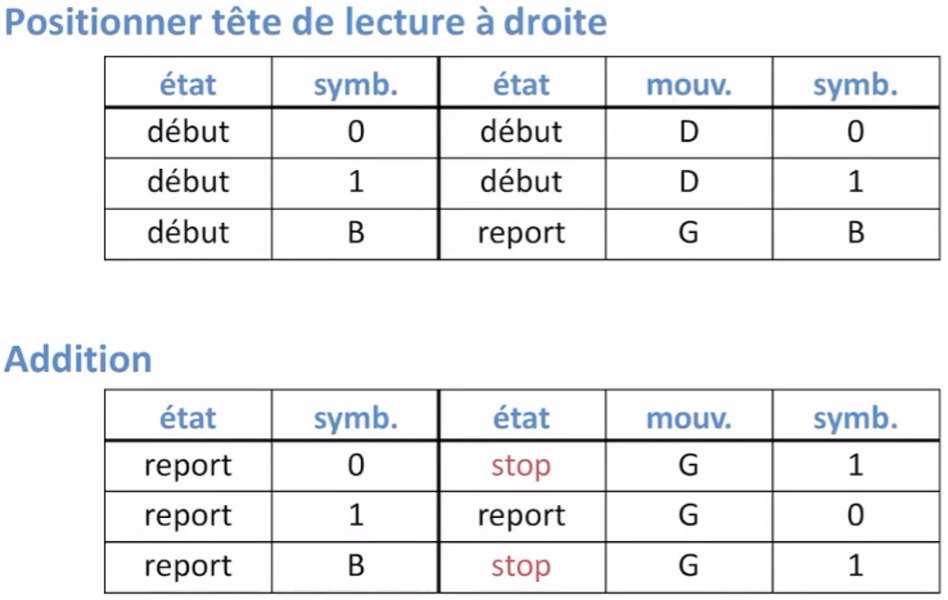
\includegraphics[width=8cm]{img/turing.png}
\caption{Tableau d'exécution pour l'addition binaire}
\end{figure}

On peut boucler en machine de Turing, par exemple on ne fait qu'aller vers la droite. Donc la machine de Turing est complet.

\subsection{Fonction T-calculables}
Une fonction f est \textcolor{red}{T-calculable} si et seulement si il existe une machine de Turing qui, recevant comme donnée (\textit{une représentation décimale de}) n'importe quel nombre naturel x, nous fournit comme résultat $f(x)$ si il est \textcolor{red}{défini}. Et ne se termine pas si $\textcolor{red}{f(x) = \perp}$\\
On peut également étendre cela aux fonctions $\mathbb{N}^n \rightarrow n$. Ce sont des définitions proche de l'idée de la calculabilité pour \textit{Java}.

\subsection{Thèse de Church-Turing}
\begin{enumerate}
\item Toute fonction T-calculable est calculable
\item Toute fonction calculable est T-calculable
\item Tout ensemble T-récursif est récursif
\item Tout ensemble récursif est T-récursif
\item Tout ensemble T-récursivement énumérable est récursivement énumérable
\item Tout ensemble récursivement énumérable est T-récursivement énumérable
\end{enumerate}
Le but de ces machines de \textit{Turing} est d'être à l'essentielle. On est à l'essence même des principes de calculabilité. De plus, la complexité est plutôt simple via le concept de transition.


\chapter{Questions Test d'entrée}

\section{TP1}
\begin{enumerate}
\item Effectivement, il existe une bijection entre les N et les nombres impairs positifs $\rightarrow$ en somme il existe une fonction qui transforme les N en impair positif
\item J'imagine qu'il y a une bijection mais je ne vois pas quel formule passant de N aux impairs existent car c'est le propre des nombres impairs 
\item Même raisonnement que la question 1
\item La fameuse formule qui lie N et Q car Q est juste une paire de N
\item Effectivement, sachant la diagonalisation de Cantor il est simple de le prouver
\item Pour N dans N il en existe une infinité et l'ensemble d'arrivé ne change pas grand-chose car on s'intéresse au nombre de fonction.
\item Effectivement, on a un nombre fini de langage donc de mot. Cela est dû grâce à l'alphabet fini et la longueur fixe. Donc on sait énumérer
\item Question typique vu au cours. En effet comme on a une infinité et il n'existe aucune bijection depuis les naturels etc.
\item Même cardinalité = bijection, il ne peut y avoir de bijection entre un ensemble non énumérable et énumérable
\item Une infinité de nombre mais effectivement même cardinalité car tous peuvent être ramené aux naturels.


\end{enumerate}

\section{TP2}
\begin{enumerate}
\item Effectivement, on ne doit pas être en capacité de coder l'algorithme pour que la fonction soit calculable.
\item Nombre premier est récursif car on a le crible d'eratosthène.
\item Si un ensemble $\textbf{X}$ est récursif (donc donne 1 ou 0) alors $\bar{X}$ l'est également car il inverse les 1 et 0.
\item Si $\textbf{X}$ est récursivement énumérable (donne 1 ou quelque chose d'autre mais pas 1) et que son opposé $\bar{X}$ est récursivement énumérable. Alors bien évidemment $\textbf{X}$ est récursif.
\item Oui, trivial.
\item Non, juste au simple fait que si $\textbf{X}$ est récursivement énumérable alors $\bar{X}$ ne peut être récursivement énumérable.
\item Vrai car on a une fonction calculable car ce sont des combinaisons linéaires de calculables.
\item Voir sous-section \ref{caract}.
\item Oui car être énumérable c'est dire qu'on peut compter tous les résultats même si ça prend un temps infini.
\item Voir sous-section \ref{caract}.
\end{enumerate}

\section{TP3}
\begin{enumerate}
\item En effet, si on a que des fonctions totales, on sait qu'on aura toujours une réponses pour n'importe quelle input.
\item Oui, le théorème de \textit{Hoare-Allison} ne dit pas l'inverse et pour le sous langage:
\begin{lstlisting}
P = return 1;
\end{lstlisting}
\item Mais si on peut avoir la fonction halt en L, on ne peut avoir sa fonction \textit{interpret}
\item Mais, on peut calculer cette fonction \textit{interpret} avec un langage de programmation qui n'est pas \textcolor{red}{restrictif}.
\item Effectivement on ne peut pas calculer toutes les fonctions totales avec L.
\item Il existe un langage qui peut calculer sa fonction halt et son interpréteur (le langage vide trivial)
\item Effectivement, ne pas être récursif n'empêche pas d'être récursivement énumérable.
\item Faux exemple: $\overline{\textbf{K}}$. (voir \ref{coreq})
\item Non, on peut imaginer 2 fonctions non récursives qui se "\textit{complètent}" et comblent les lacunes de chacune. Exemple: $K \text{ et } \overline{K}$
\item Non, on peut imaginer une intersection qui ne comportent que des entrées avec une réponse.
\end{enumerate}

\section{TP4}
\begin{enumerate}
\item Faux, l'ensemble des programmes qui ont pour fonction $2n$ est non récursif car notre ensemble à toutes les fonctions qui ont ce résultat.
\item Faux, car on possède toutes les fonctions qui renvoient $0$ pour n'importe quelle entrée.
\item Vrai, car certains programmes peuvent hors de notre ensemble ont la même fonction. C'est le \textit{1000 instructions} qui posent soucis. Car des programmes qui en ont + peuvent retourner le même résultat.
\item Faux, en effet un programme qui prend 3 entrées (donc hors de notre ensemble) a le même résultat qu'un faisant partie de notre ensemble. Et ceci est valable pour \textbf{tous} programmes dans notre ensemble.
\item Cela dépend de la fonction f, en effet, même sorte de raisonnement que pour le 4. donc cela dépend. On peut aussi avoir des fonctions non calculables.
\item Il faudrait tester toutes les entrées pour en être sûr donc $\mathbb{N}$.
\item Oui, voir l'idée avec halt, ...
\item C'est l'ensemble formé par Halt donc pas récursif.
\item Mais c'est bien récursivement énumérable comme Halt.
\item Non, il faut faire une réduction à halt.
\end{enumerate}

\chapter{Question cours}
\section{S1}

\section{S2}
Une densité du nombre de rationnel
Un langage est un ensemble de chaine de caractère ! Attention de ne pas confondre langage le mot vulgaire et langage en informatique.\\
Fonction totale s'intéresse au domaine.\\
Fonction surjective s'intéresse à l'image.\\
\begin{itemize}
\item Injective max une flèche.
\item Surjective min une flèche.
\item Étendre une fonction est rajouté une flèche.
\end{itemize}

\section{S3}
Attention à la notation entre$ \rightarrow P_{12} \neq P_{47}$ car $P$ sont des chaines de caractères bien déterminés et donc différentes
$\varphi_{12}=\varphi_{47}$ effectivement car phi est créé depuis des P différents mais peuvent créer des fonctions donnant le même résultat\\

$Halt(n,37)$ n'est pas calculable car si ce serait, halt serait calculable\\
Print(1) car tous les Entiers appartiennent à $\mathbb{N}$\\

Recursif: calculable
Récursivement énumérable: calculable et ne dit pas s'il ne l'est pas.

\section{S4}
Différence entre Q et JAVA, toutes les fonctions se terminent et rendent une valeur. 
Java lui peut rendre une fonction bottom !
Donc notre démonstration ne fonctionne plus car $interpret(k,k)= \perp$ et donc $diag_{mod}= \perp+1= \perp$\\

Est-ce le fait qu'un interpréteur ne puisse être écrit en Q problématique ?
Un interpréteur prend en entrée un code et met des mots-clés. L'interpréteur va créer un arbre d'exécution.\\
SQL est un langage qui ne boucle jamais. $\rightarrow$ Donc SQL ne peut être utiliser pour faire des programmes complexes.\\

Impossible de détecter les cas sans réponses. (fonction HALT en exemple)

\section{S6}
\begin{enumerate}
\item Pourquoi la propriété S est-elle une conséquence du théorème S-m-n ? Avec le théorème S-1-1 Il existe une fonction totale calculable $S_1^1:N^2\rightarrow N$
\item Lesquelles de ces affirmations sont vraies
\begin{enumerate}
	\item Si f est une transformateur de programmes (f fonction totale calculable), alors il existe deux programmes P1 et P2 tels que $f(P1) = P2$ ainsi que P1 et P2 calculent la même fonction  Le théorème de u point fixe
	\item Si f est une transformateur de programmes (f fonction totale calculable), alors il existe deux programmes P1 et P2 tels que f(P1) = P2 ainsi que P1 et P2 calculent la même fonction totale $\rightarrow$ le totale nous force à avoir quelque chose qui se termine toujours
\end{enumerate}
\item À quoi sert le théorème du point fixe:
\begin{enumerate}
\item Faire un programme qui sans paramètre donne son propre code en sortie standard
\end{enumerate}
\item Post $\rightarrow$ impossible même avec Bruteforce. Diophantienne $\rightarrow$ l'utilité est minime.
\item Nombre réels non-calculables est-elle une conséquence immédiate du fait que R est non énumérable.
Donne un output fini aussi précis que je le voudrais. R n'est pas énumérable et j'ai un nombre énumérable de programme donc je ne peux pas représenter tous les R.
\end{enumerate}

\section{S7}
\begin{itemize}
\item \textcolor{blue}{Sémantique}: signification du programme et sa fonction calculé
\item \textcolor{blue}{Syntaxique}: comment écrire correctement le programme et qu'il soit compréhensible par l'ordinateur
\end{itemize}

Si un ensemble A est ND-récursif, les différentes exécutions du programme ND-Java qui décide cet ensemble doivent-elles nécessairement se terminer pour chaque input possible.$\rightarrow$ ce sont des arbres de décisions (accepter les résultats si oui ou non etc)\\

Tant qu'une façon d'avancer dit oui même avec une boucle infini, on peut accepter.\\
Quel est le but d'un langage non déterministe car pas exécutable sur un pc? Car sinon on va saturer et on n'aura pas assez de cœur et on passera en séquentiel. (ex: parcours en largeur): C'est pour modéliser des problèmes\\

Avec BLOOP je peux calculer des choses mais pas toutes les fonctions totales et calculables (hoare allison)\\

Automate fini chose simple qui répète toujours la même chose en boucle sans dépendre du passé.\\

Par hoare allisson que les automates sont toujours finis et s'arrête\\

Si on a une façon acceptante, on peut toujours l'accepter et dire oui.\\

On ne peut pas programmer toutes les fonctions calculables en automate fini

\chapter{Vrai ou Faux cours} %améliorer la mise en page
Cette section regroupe toutes les réponses et raisonnements des questions \textbf{wooclap} posées au cours.

\section{S1}
Introduction donc pas de QCM.

\section{S2}
\textcolor{red}{Besoin de contributeurs}
Je n'ai pas noté :(( 
%ajoutez le questionnaire

\section{S3}
%ajouter les questions pas que les réponses
\textcolor{red}{TODO ajouter les questions pas que les réponses}

\begin{enumerate}
\item Tout language n'est pas récursif car c'est un ensemble de fonction dont Halt qui n'est pas récursif
\item Tout ensemble énumérables n'est pas récursif.
\item Un ensemble fini est récursif
\item Le complément d'un ensemble récursif est récursif
\item L'ensemble des rationnels est récursivement énumérable
\item Un sous-ensemble infini d'un ensemble récursivement énumérable n'est pas récursivement énumérable
\item Un sous-ensemble fini d'un ensemble récursivement énumérable n'est pas récursivement énumérable
\item L’union d’une infinité énumérable d’ensembles récursivement énumérable n'est pas récursivement énumérable: Exemple avec l'ensemble K
\item Le complément d’un ensemble récursivement énumérable n'est  pas récursivement énumérable: Exemple avec K et inverse de K
\item Une fonction dont la table est infinie est calculable
\item Un algorithme ne calcule qu'une et une seule fonction
\item Il existe des ensembles non récursivement calculable
\item Une fonction calculable est peut être calculée par une infinité de programmes
\item L'ensemble HALT n'est pas récursivement énumérable
\item Il existe des ensembles récursifs qui sont récursivement énumérables
\item Il existe des ensembles récursifs qui ne sont pas énumérables
\item Si le domaine d'une fonction est finie, alors cette fonction est calculable: on peut faire une liste de tous les cas possibles
\item Si le domaine de fonction est infini, alors cette fonction est calculable
\end{enumerate}

\section{S4}
\begin{enumerate}
\item Il existe un langage non trivial dans lequel la fonction halt est calculable. $\rightarrow$ on sait que tout ce fini en Q donc oui on sait calculer halt car c'est la fonction constante 1 (non trivial $\rightarrow$ pas les réponses facile type langage vide)
\item Il n'existe pas un langage de programmation (non trivial) dans lequel on peut programmer le fonction halt ainsi que l’interpréteur de ce langage
\item Si un langage de programmation (non trivial) permet de programmer son interpréteur, alors la fonction halt n'est pas calculable dans ce langage
\item Il existe de langage de programmation (non trivial) dans lequel toutes les fonctions calculées sont totales
\item Il n'existe pas un langage de programmation ne permettant de calculer que des fonctions totales, mais toutes les fonctions totales calculables $\rightarrow$ l'interpréteur ne peut pas être calculé en Q
\item il n'existe pas une fonction totale calculable qui n'est l'extension d'aucune fonction partielle calculable $\rightarrow$ effectivement car on a une fonction calculable totale elle est d'office l'extension d'une fonction partielle calculable.
Il existe une fonction partielle calculable telle qu’aucune fonction totale calculable n’est une extension de cette fonction partielle --> énoncé du théorème, pas de messages d'erreur.
\end{enumerate}

\section{S5}
\begin{enumerate}
\item L'ensemble des programmes Java calculant une fonction $f$ telle que $f(10) = 10$ n'est pas récursif (car ici on caractérise que fait le programme !)
\item L’ensemble des programmes Java calculant une fonction $f$ telle que $f(10)=10$ est un ensemble récursivement énumérable. (n'a aucun rapport avec Rice !!!)
\item Toute propriété relative aux programmes est calculable (théorème de rice parle des propriétés calculés par la fonction pas lié à la fonction
\item Si A est un sous-ensemble (strict et non vide)  récursif de programmes Java, alors toute fonction calculée par un programme de A n'est pas aussi calculée par un programme du complément de A (car il existe pas qu'il existe pour tout !!!)
\item Soit la fonction $revenu1_yde(n) =$ le revenu imposable de Yves Deville à l'année $n$.  Si n est inférieur à $1960$ ou supérieur à $2060$, le résultat de cette fonction est $\perp$. Par hypothèse, une personne décédée a un revenu de $0$.  Cette fonction est-elle calculable ? (Car n'est définie que pour $101$ inputs. Calculable car nb fini de point à calculer. Domaine finie == calculable au sens théorique du terme)
\item Soit la fonction $revenu2_yde(n) =$ le revenu imposable de Yves Deville à l'année $n$. Par hypothèse, une personne pas encore née ou décédée a un revenu de $0$. Cette fonction est-elle calculable ? ( car est constante sauf pour un certain input. Ici on n'est jamais bottom donc il existe toujours une fonction)
\item Un programme Java étant fini, l’exécution de ce programme sera aussi finie (car il peut boucler)
	Soient les programmes $P_32$ 
\item (n) dont le code est « print(1) » et $P_57(n)$ dont le code est « print(0) ».  Cochez les affirmations correctes (on peut pas varier de l'un à l'autre)
\item Une extension d’une fonction partielle calculable est toujours calculable (faux car il existe des fonctions qui ne peuvent être étendue ex: HALT)
\item L’ensemble des sous-ensembles des entiers est énumérable (car autant que les réelles, on a besoin d'une chaine infinie de caractère)
\item Il existe un ensemble infini de chaînes finies de caractères (A-Z) qui est non énumérable (on peut créer des chaines de caractères de chiffres et ce sera fini)
\item Il existe un ensemble infini de chaînes finies de caractères (A-Z) qui est non récursivement énumérable (ensemble non récursif $\rightarrow$ complément K $\rightarrow$ c'est une représentation
\item La fonction $halt(18,x)$ est calculable (cela dépend de la numérotation choisie des programmes Java)
\item L'ensemble des fonctions non calculables est énumérable (Faux car infinité)
\item Soit A est un ensemble (infini) récursivement énumérable.  Si $ B \subseteq A $, alors $B$ est aussi récursivement énumérable. (Faux car le sous-ensemble peut prendre que des choses bottoms)
\item Il existe des langages de programmation (non triviaux) dans lesquels toutes les fonctions calculées sont totales (Vrai, mini-Java ne calcule que des fonctions totales et calculables. Toutes les fonctions sont totales)
\item Si une fonction $f$ est calculable, alors toute fonction g dont f est une extension est calculable (Faux, $\rightarrow$ le théorème de l'extension parle pas de ça. Car g peut être bottom et donc ne pas être calculable (genre 1 si élément appartient au complément de $K$ ou $\perp \rightarrow$ fonction pas calculable et $f$ est une extension))
\item Soit le programme numéro n calculant la fonction factorielle ($f(x)=x!$ si $x$ non négatif et $f(x)=\perp$ si $x$ négatif,).  Cochez les affirmations correctes:
	\begin{enumerate}
	\item $\varphi_l(n)$ calcule bien quelque soit l'énumération choisie pour les programmes
	\item Pas énumération car n est positif
	\item Une infinité de programmes calculent la même fonction
	\item Par hasard
	\item Pas injectif car ne fait d'office correspondre au max $1$ une fois. (penser à $0!$ Et $1!$ Même réponse)
		\end{enumerate}

\end{enumerate}

\section{S6}
\begin{enumerate}
\item La propriété S-m-n affirme que tout numéro de programme calculable peut être transformé en un numéro équivalent, mais avec moins de paramètres $\rightarrow$ \textcolor{red}{Faux}, on transforme un programme en un autre programme. Les fonctions sont équivalentes.
\item Les propriétés S-m-n et S  sont équivalentes $\rightarrow$ \textcolor{red}{Faux}, S-m-n implique S mais pas dans l'autre sens.
\item Tous les langages de programmation (standards) satisfont la propriété S-m-n, on peut spécialiser un programme par ses arguments
\item Le théorème du point fixe est une conséquence du théorème de Rice $\rightarrow$ \textcolor{red}{Faux} c'est l'inverse
\item Si deux programmes P1 et P2 calculent la même fonction, alors il existe un transformateur f de programmes (f  fonction totale calculable) , tel que f(P1)=P2 $\rightarrow$ \textcolor{green}{Vrai}, ce n'est pas le théorème du point fixe. On a 2 programmes qui calculent la même fct, on une fct qui transforme P1 et P2 (return P2)
\item Si f est un transformateur de programmes (f  fonction totale calculable),  alors il existe deux programmes P1 et P2 tels que f(P1)=P2 ainsi que  P1 et P2 calculent la même fonction $\rightarrow$ \textcolor{green}{Vrai} énoncé du point fixe mais un peu moins math.
\item Si f est un transformateur de programmes (f  fonction totale calculable),  alors il existe deux programmes P1 et P2 tels que f(P1)=P2 ainsi que  P1 et P2 calculent la même fonction totale $\rightarrow$ \textcolor{red}{Faux}, attention au totale, on n'exige pas que les programmes s'exécutent toujours.
\item Le théorème du point fixe permet de démontrer que la fonction halt  est non calculable $\rightarrow$ \textcolor{green}{Vrai}, pt-fixe donne halt
\item La non calculabilité du problème de Post est une conséquence du théorème de Rice $\rightarrow$ \textcolor{red}{Faux}, c'est une autre famille de problème non calculables, c'est lié au problème des chaines de caractères
\item L’ensemble des nombres réels calculables est énumérable $\rightarrow$ \textcolor{green}{Vrai} car on l'approche via un programme et le nombre de programme est calculable
\item Il existe une infinité non énumérable de nombres réels non calculables $\rightarrow$  \textcolor{green}{Vrai} les réels calculables sont énumérables donc l'ensemble opposé doit être non énumérable sinon ça voudrait dire que les réels sont énumérables.
\end{enumerate}

\section{S7}
\begin{enumerate}
\item Toutes les fonctions calculables par les programmes du langage BLOOP sont totales $\rightarrow$ \textcolor{green}{Vrai} toujours terminé donc tot
\item Le langage BLOOP (Bounded Loop) ne permet de programmer que des fonctions totales.  Il existe donc des fonctions totales calculables qui ne peuvent être programmées dans ce langage. $\rightarrow$ \textcolor{green}{Vrai} hoare allison
\item Les langages non déterministes permettent d’écrire des algorithmes plus efficaces. $\rightarrow$ \textcolor{red}{Faux}, plus simple de les exécuter mais on ne peut pas exécuter tout en parallèle
\item Tout ensemble ND-récursivement énumérable  est récursif $\rightarrow$ \textcolor{red}{Faux}, ND et déterministe est la même chose. Cela n'apporte rien en calculabilité. ND facilite la description de problème. Donc est-ce un ensemble récursivement énumérable récursif ? Faux bien évidement
\item Il existe des ensembles récursifs ne pouvant être décidés par un automate fini $\rightarrow$ \textcolor{green}{Vrai}, HOARE ALLISON ! Tous les programmes se terminent 
\item Tout automate fini non déterministe peut être transformé en un automate fini déterministe équivalent $\rightarrow$ \textcolor{green}{Vrai}, un programme non déterministe Java peut être transformé en déterministe en faisant étape par étape
\end{enumerate}

\end{document}
